\chapter{相关技术研究}
随着互联网技术的发展与国民生活水平的提高,手机持有率直线上升,
手机网民大规模增长,人们在网上产生的信息、发布的文本日益碎片化。
为了有效利用这些片段化的信息,短文本分类技术,作为自然语言处理的关键技术之一,
得到了充分的关注与发展,
短文本分类应用的影子在互联网中随处可见。
本章将对传统文本分类技术进行论述,并介绍本文涉及到的相关技术问题。
\section{中文文本分词}
\label{word_seg}
词是最小的能够独立活动的有意义的语言成分,在英文文本中,每个单词天然的由空格分割开来,
使得研究人员可以毫无难度的获取文本中所有的单词,然后进行接下来的研究工作。
但对于中文这样由字组成的连续文本,并不存在这样的语言优势,词语之间没有明确的区分标记,
要想进行语义分析,必须先将中文文本切分,因此中文分词是中文信息处理的基础和关键。
同时,大量实验表明,分词的好坏直接关系着后续分类算法的最终效果,所以选择一个快速并
准确的分词算法尤为重要。目前常用的分词方法主要有两大类:基于字符串匹配的算法与基于规则的算法。
\subsection{基于字符串匹配的分词算法}
基于字符串匹配的分词算法又称为机械分词算法,主要依据外部提供的词典,
按照一定的策略将待切分的中文文本与词典中的词条逐一匹配,
若在词典中找到该词条,则匹配成功并切分为单词,否则做其它相应的处理。
查找词库的匹配策略分为两种:长单词优先的最大匹配法以及短单词优先的最小匹配法。
在实际使用中,人们发现单词切分次数越短,切分出的单词越长,分词效果越好,
所以目前一般使用最大匹配法。
按照匹配顺序的不同,最大匹配算法又可分为:正向最大匹配算法\citing{张劲松2009回溯正向匹配中文分词算法}、
逆向最大匹配算法\citing{李娟2010一种改进的逆向匹配快速切分算法}、
双向最大匹配算法\citing{陈耀东2005基于有向图的双向匹配分词算法及实现}。

(1)正向最大匹配算法

正向最大匹配算法的基本思想是:已知词典中最长单词的长度为$N$,则以$N$最为截取单词初始长度。
对于带切分的中文文本$S$,首先从左向右截取长度为$N$的字符串$W_{1}$,
然后在词典中寻找是否有和该字符串$W_{1}$匹配的单词。如果找到,则将$W_{1}$标记为成功切分出的单词,
再继续从待切分文本的$N+1$处开始下一次匹配;如果没找到,则将截取长度减$1$重新截取,即在$S$的原来位置重新截取长度为$N-1$的字符串,
然后重复之前匹配操作,直到截取长度为$1$。算法流程如图\ref{max_match}所示:

\begin{figure}[h]
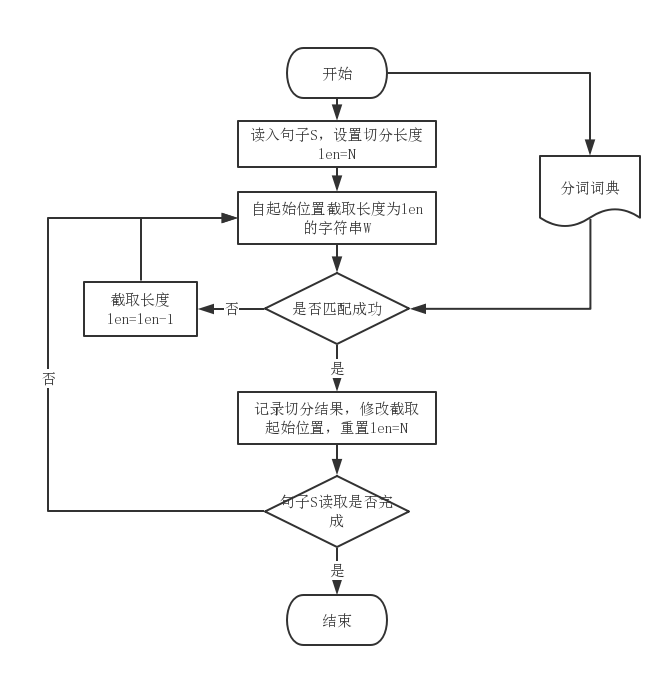
\includegraphics[scale=0.6]{picture/max_match.png}
\caption{正向最大匹配算法流程}
\label{max_match}
\end{figure}

(2)逆向最大匹配算法

逆向最大匹配算法思路和正向最大匹配算法大致相同,不同之处在于截取字符串时的方向由从左向右换成了从右向左。
也就是说,当对句子分词时,根据词典中最长单词的长度,从句子末尾开始向左截取字符串与词典中的
单词匹配,直到切分到句子的开始位置为止。

(3)双向最大匹配算法

双向最大匹配算法是上述两种最大匹配算法的结合,侧重于分词过程中的检错和纠错,其基本思路是对待分词文本分别
采用正向最大匹配和逆向最大匹配进行初步切分,然后将得到的正向分词结果和逆向分词结果进行比较,如果
两种方法的结果一致,则认为分词结果正确,如果结果存在出入,则认为分词存在着切分错误,需要采用其他技术手段消除
结果中的歧义。

从上面的分析可以明显看出,无论哪种最大匹配算法都极度依赖词典,只有在词典覆盖的领域内,才有较理想
的分词效果。对与词典没有覆盖的陌生领域语料,极端情况下甚至会出现单字切分的分词结果。

\subsection{基于统计的分词算法}
\label{subsection:n_girm}

这类分词算法并不依赖具体的词典,而是根据语料中的统计信息,识别句子中的单词。即把单词看做是
特定的字的结合,在语料中邻近的字共同出现的次数越多越可能是一个词。所以计算句子中特定字的组合的出现概率,
可以判断这个组合是否是一个词。通过以概率论为理论基础,将中文文本中的每一个词的出现抽象成随机过程,
分词算法不会被待分词文本的内容所影响,对所有领域的中文语料都有统一的效果,
这是极度依赖词典的基于字符串匹配的分词算法所没有优势。根据采用的统计模型不同,基于统计的分词算法
又可分为互信息算法、N元统计模型等。

(1)互信息算法

在概率论和信息论中,两个随机变量的互信息是这两个变量彼此之间依赖性的一个度量。更确切的说,它是根据另一个
随机变量来量化一个随机变量中可以获得的信息量。互信息分词算法是互信息理论在分词中的应用,通过计算
两个相邻字符串的互信息值,来判断它们之间的结合程度(即组成一个单词的可能性)。

对于两个相邻字符串$x$和$y$,它们的互信息值计算公式如下:
\begin{equation}
    I\left ( x,y \right )=\log \frac{p\left ( x,y \right )}{p\left ( x \right )p\left ( y \right )}
\end{equation}

其中$p\left ( x,y \right )$表示字符串$x$和$y$在语料中共同出现的频率,$p\left ( x \right )$与$p\left ( y \right )$分别表示字符串$x$与$y$的出现频率。
当$I\left ( x,y \right )>0$时,表示$x$和$y$具有一定的相关性,并且这个值越大,它们联系的就越紧密,
超过某一个阈值时即可判定为一个词;当$I\left ( x,y \right )=0$时,表示$x$和$y$的关系不明确;当$I\left ( x,y \right )<0$时,表示$x$和$y$直接几乎没有相关性,
基本不会组成一个词。

(2)N元统计模型

N元统计模型又称为N元语言模型(n-gram language model),本质上是对语言建模的一种统计模型。
该模型假定语言满足马尔科夫性,句子中的单词的出现与其前面出现的单词紧密相关,即第$n$个词的出现
只与前面$n-1$个词的出现相关,而和其他任何词都不相关。假设句子$S$由单词序列$\left (w_1,w_2,...,w_m  \right )$组成,
则N元语言模型可表示为:
\begin{equation}
    \begin{aligned}
        P\left ( S \right )&=P\left ( w_1w_2...w_m \right )\\
        &=P\left ( w_1 \right )P\left ( w_2|w_1 \right )...
P\left ( w_i|w_{i-n+1}...w_{i-1} \right )...P\left ( w_m|w_{m-n+1}...w_{m-1} \right )
    \end{aligned}
    \label{n-gram}
\end{equation}

理论上来说,$N$取值越大,模型就越精确,越能揭示出语言的内在结构。但随着$N$的增加,模型的计算复杂度也呈几何式上升,
所以在实际应用中,通常将$N$取值为2、3、4,而$N$取2的N元统计模型称为bigram模型,$N$取3的则称为trigram模型。

在分词应用中,算法首先对句子$S$进行全切分,得到若干分词结果,再根据公式\ref{n-gram}计算这些分词结果的概率$P\left ( S \right )$,
最后选择概率最高的分词结果作为最终结果。

\section{传统文本表示方法}
分词处理之后,文本信息转化为一个单词序列,但对于计算机与程序来说依然是一段没有意义的字符串。
为了让程序能够理解文本信息,继续之后的分类工作,我们需要对其再次处理,提取出其中的有效信息,将字符串文本
映射成结构化的数字信息。

\subsection{向量空间模型}

向量空间模型(Vector Space Model,VSM)最早由Salton等人\citing{薛苏琴2016基于向量空间模型的中文文本相似度的研究}于20世纪70年代提出,
是一种将文本信息表示为向量的代数模型。模型的主要思想是将文本看做单词的简单组合,通过
统计语料中不同单词的个数,构建一个$n$维的向量,向量中每一个纬度都代表一个不同的单词,单词在文本中存在,则此位为$1$,否则为$0$,以此将一段文本信息
转换为一个$n$维的数学向量。

可以明显看出,虽然向量空间模型建立了一个从文本到向量的快速转换,让程序能够容易地对文本进行处理计算,
但这种映射方式太过简单。将文本表示为单词的组合,忽略了词语的位置关系以及词语之间的相互联系。把相同单词都统计为一类,
也忽略了一词多义的情形,让程序难以进行进一步的语义分析。而且,当统计的语料足够多后,
模型产生的向量会拥有一个巨大的维度,造成后续计算的维度灾难。

为了解决上述问题,实际使用中,通常使用文本的关键词作为文本向量,而不是使用所有单词。因此,如何选择关键词就变得尤为重要。

\subsection{TF-IDF特征提取}

TF-IDF(term frequency–inverse document frequency)是一种常用的关键词提取技术,
它表明了一个词对于语料库中一份文本重要程度。算法的中心思想是:一个词的重要性与它在文本中出现的次数成正比,但同时
也与它在整个语料库中出现的次数成反比,即如果某个词在一份文本中出现频率很高,同时在语料库中其他文本中
出现频率很少,那么就认为这个词对于这份文本非常重要。

在TF-IDF中,TF(term frequency)代表词频,对于文本$j$的单词$i$,它的TF值可以通过公式\ref{tf_equ}计算。
\begin{equation}
    TF_{i,j}=\frac{n_{i,j}}{\sum_k n_{k,j}}
    \label{tf_equ}
\end{equation}
其中$n_{i,j}$表示单词$i$在文本$j$中出现的次数,$\sum_k n_{k,j}$表示文本$j$中所有单词的出现次数之和。

IDF(inverse document frequency)代表逆文档频率,是对一个词可以提供的信息量的一个度量,可以体现这个词
在所有文档中是否重要。详细的计算方法如公式\ref{idf_equ}所示。
\begin{equation}
    IDF_{i,D}=\log \frac{\left | D \right |}{1+\left | \left \{ d\in D:t\in d \right \} \right |}
    \label{idf_equ}
\end{equation}
其中$\left | D \right |$表示语料库中的文本总数,$\left | \left \{ d\in D:t\in d \right \} \right |$表示包含单词$i$的文件数量。

最后,根据公式\ref{tf_equ}和\ref{idf_equ}可以得到单词$i$的TF-IDF值,如公式\ref{tf_idf_equ}所示。
\begin{equation}
    TF-IDF_{i,j}=TF_{i,j} \cdot IDF_{i,D}
    \label{tf_idf_equ}
\end{equation}

\section{传统文本分类方法}
传统文本分类方法使用机器学习中的分类器对文本特征向量进行分类,这类分类器本质上是
通过设定一个能够将任何特征向量映射到某一具体类别的理想目标函数$\gamma$($\gamma :D\rightarrow C$),
然后根据学习算法减少自身的误差不断接近目标函数,最终实现分类的目的。按照设定的目标函数的不同,
分类器可以分为线性分类器与非线性分类器,下面将对几种常见分类器作简要介绍。
\subsection{贝叶斯分类器}
朴素贝叶斯分类器\citing{mccallum1998comparison}是一种典型的线性分类器,并且也是最古老及最简单的分类器之一。
朴素贝叶斯理论是该分类器的基本理论,它在分类任务中对输入数据有一个基本假设:数据的各特征之间是条件独立的。
虽然这个假设看起来可能明显是错的,但依据朴素贝叶斯理论实现的朴素贝叶斯分类器在结构化或半结构化数据上都有比较理想的表现。
同时,朴素贝叶斯分类器对CPU和内存的消耗也少于其他分类器。

朴素贝叶斯理论是指在上面提到的基本假设下,对于事件$A$和$B$,它们之间的概率关系满足公式\ref{bayes}。
\begin{equation}
    P\left ( A | B\right )=\frac{P\left ( B | A\right )P\left ( A \right )}{P\left ( B \right )}
    \label{bayes}
\end{equation}
而在文本分类任务中,假设一篇文本的特征向量为$D=\left \{ d_1,d_2,...,d_m \right \}$,它的类别为$C$,则上式可以写为公式\ref{bayes_text}。
\begin{equation}
    P\left ( C | D\right )=\frac{P\left ( D | C\right )P\left ( C \right )}{P\left ( D \right )}
    \label{bayes_text}
\end{equation}
其中$P\left ( C \right )$和$P\left ( D \right )$是先验概率(prior probability),分别表示类别$C$和特征向量$D$出现的概率,
$P\left ( D | C\right )$代表在类别$C$中出现特征向量$D$的概率,$P\left ( C | D\right )$则是分类器
的结果,称为后验概率(posterior probability),代表特征向量$D$是类别$C$的概率。实际应用中,
$P\left ( C \right )$和$P\left ( D \right )$以及$P\left ( D | C\right )$都可以根据训练语料库
直接计算得到。

\subsection{支持向量机}
支持向量机(Support Vector Machine,SVM)是感知机的一种改进算法,在机器学习算法中有非常广泛的应用。

在感知机模型中,分类器通过寻找一个可以将数据正确分为两类的超平面来实现二元分类任务。但是,如图\ref{separating_lines}所示,这样的
超平面往往不是唯一,并且不同的超平面选择会导致感知机的分类准确率截然不同。
\begin{figure}[h]
    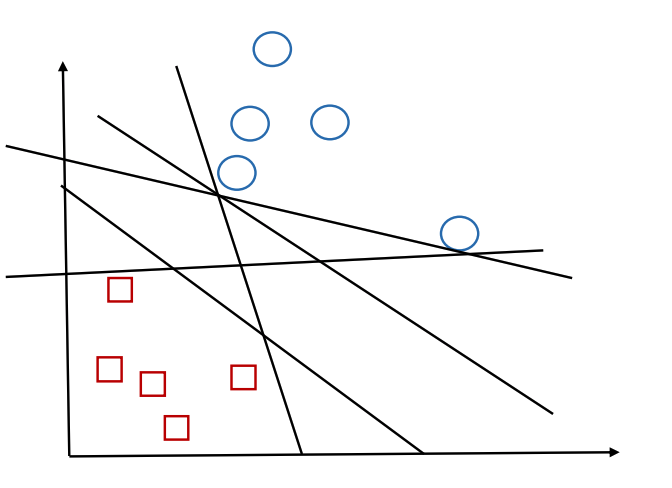
\includegraphics[scale=0.4]{picture/separating-lines.png}
    \caption{超平面示意图}
    \label{separating_lines}
\end{figure}

为了选择一个分类效果最佳的超平面,支持向量机将距离超平面最近的点设定为支持向量,然后让这些支持向量和超平面
之间的距离最大,从而选择出一个最优的超平面,如图\ref{svm}所示。并且对于线性分类不适用的非线性数据(如文本数据),支持向量机利用
核函数的技巧,通过选择一个恰当的转换函数,将非线性数据映射到一个更高维的向量空间当中,让数据重新分布为线性可分的形式。
但是这种做法增加了算法复杂度,复杂的核函数会使算法的计算量成倍的提高,而且如何选择合适的核函数让数据线性可分也没有一个统一
的方法。
\begin{figure}[h]
    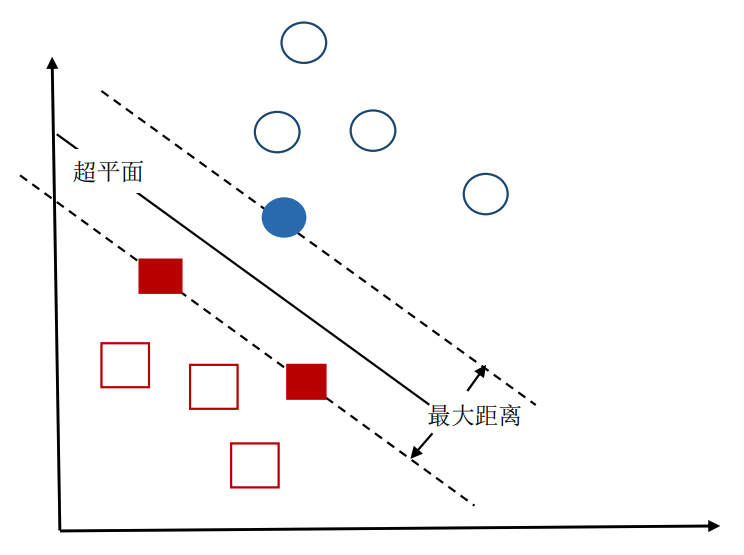
\includegraphics[scale=0.35]{picture/svm.png}
    \caption{支持向量示意图}
    \label{svm}
\end{figure}

\section{基于神经网络的短文本分布式表示方法}
\label{sect_word2vec}
传统文本分类方法虽然在篇章级的长文本上能够有较好的分类效果,
但是对于文本信息量较少的短文本来说,却难以发挥效用。基于统计的
特征提取方法会在训练时生成庞大的特征词库,文本特征向量的维度依然很高,一旦文本长度过短,
特征向量就会变为稀疏向量,即数据只集中在向量中的某几维上,其他维度都为零。
文本特征向量的稀疏性一直是短文本分类上最难以解决的问题之一,为了解决这个难题,学者们开始
尝试引入神经网络与深度学习技术。

短文本的分布式表示方法也称为词向量表示法,在神经网络与深度学习模型中,输入数据通常需要转化为矩阵的形式。对于自然语言处理任务,则需要
将文本中的词语表示为一个向量,从而让模型理解文本并进一步提取特征,完成分类任务。

One-hot Representation是词向量表示法最简单的实现方式,具体方法与前文中介绍的向量空间模型
大致相同,针对具体语料可以快速得到每个单词的词向量。但与向量空间模型一样,存在维度过高与稀疏性的问题,
并且从词向量之中无法得到词语之间的关系,对短文本分类任务并不适用。

为了得到连续稠密的词向量,Hinton等人提出了一种称之为词嵌入(Word Embedding)的词向量实现方法\citing{hinton1986learning}。
该方法旨在根据语料库中词语的分布式属性,来量化不同词语之间的语义相似度。
通过一系列转换函数,将词语从高纬度文本空间映射到一个维度相对较低的向量空间,表示为低维实数向量,
从而有效的解决了向量的稀疏问题。并且这种映射方法还保留了词语之间的关系,
即意思相近的词语它们产生的词向量也会在向量空间中彼此靠近。

目前最常用的词向量构建工具是word2vec,由Google公司于2013年发布\citing{mikolov2013distributed}。
该工具基于\ref{subsection:n_girm}中介绍的N元语言模型思想,假定文本中的一个单词只和其相邻的N(word2vec中称为窗口大小)个单词相关,
构建了两套词向量模型——CBOW模型及Skip-gram模型。

CBOW模型仿照神经网络语言模型的思想(Neural Network Language Model,NNLM),
根据目标词的上下文环境来预测目标词,如图\ref{cbow}所示。
\begin{figure}[h]
    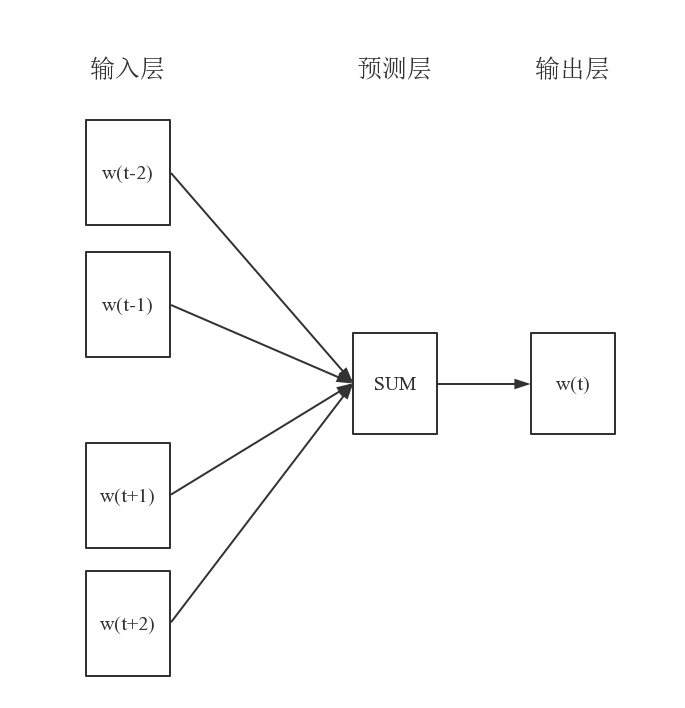
\includegraphics[scale=0.6]{picture/cbow.png}
    \caption{CBOW模型}
    \label{cbow}
\end{figure}

不同的是,CBOW删除了NNLM中前向反馈神经网络的隐藏层,将中间层直接和输出层的softmax节点连接,
并且忽略了目标词上下文的顺序信息,把输入的全部词向量都汇聚在同一个隐藏层节点上。
因此从数学上看,CBOW模型相当于是把一个词袋模型的向量乘以一个嵌入矩阵,来得到一个连续的词嵌入向量。

与CBOW模型相反,Skip-gram模型的思想是根据目标词预测与目标词相邻的单词,
模型结构如图\ref{skip-gram}所示。
\begin{figure}[h]
    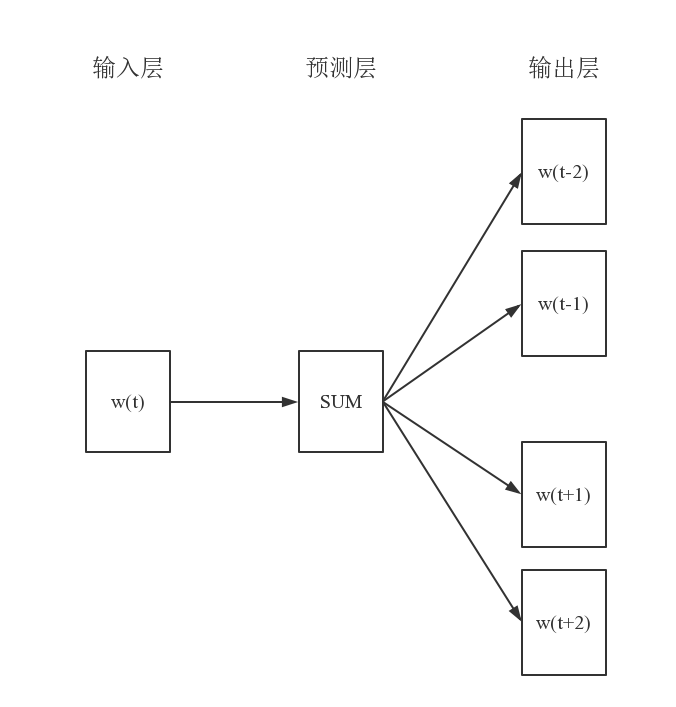
\includegraphics[scale=0.6]{picture/skip-gram.png}
    \caption{Skip-gram模型}
    \label{skip-gram}
\end{figure}
对于句子$S$,Skip-gram模型的目标函数如式\ref{skip-gram_eqn}所示。
\begin{equation}
    \arg \max_{\theta } \prod_{\left ( w,c \right )\in S}p\left ( c|w;\theta \right )
    \label{skip-gram_eqn}
\end{equation}
其中$w$为目标词,$c$为目标词$w$周围的一些单词,长度由模型的窗口大小决定,$\theta$是隐藏层参数。

word2vec工具的优点主要体现在计算快速,通过简化传统NNLM的结构,引入分层softmax(Hierarchical softmax)和
负采样(Negative Sampling)技术,极大的减少了预测层到输出层之间的计算量。
同时模型采用非监督训练,适用于无标签的大型语料库。

word2vec工具的缺点也十分明显:
针对英语的设计,只使用单词信息进行训练,使得模型不能够理解单词内在的一些语义信息。
因此本文在原始CBOW模型之上,增加中文的字和偏旁部首信息,致力于实现一个适用于中文的
词向量模型。

\section{基于神经网络的短文本分类方法}
与传统文本分类方法不同,基于神经网络的短文本分类方法使用更为复杂的
深度学习网络来提取文本特征,从而克服传统特征提取算法在短文本上的不足。
分类网络的一般框架如图\ref{classification_net}所示,
整体使用端到端训练(end-to-end training)\citing{chan2016listen}的方式
,以短文本的词向量矩阵作为输入数据,使用相应的特征提取网络从中提取语义特征,
得到文本特征向量,然后输入多类别分类器进行分类,最后与标注数据对比完成网络的训练。
本小结主要介绍两种常见的用于提取文本特征的深度学习网络。
\begin{figure}[h]
    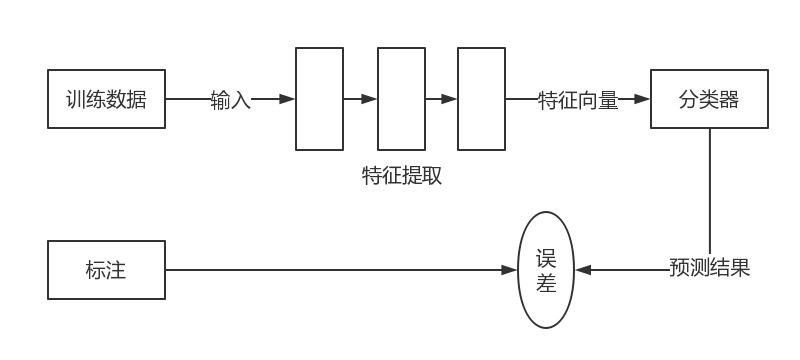
\includegraphics[scale=0.5]{picture/classification_net.png}
    \caption{短文本分类网络的一般结构}
    \label{classification_net}
\end{figure}


\subsection{卷积神经网络}
\label{cnn_section}
卷积神经网络(Convolutional Neural Network, CNN)\citing{lecun1989backpropagation}是一种前馈神经网络,
通过模仿猫脑皮层中用于局部感知和方向选择的神经元结构,有效降低了普通反馈神经网络的复杂性。

文本分类任务中,普通的神经网络模型通过构建一个全连接的网络对句子进行处理,
输入层的神经元直接接收文本的词向量,计算时隐藏层的某些节点会被输入的特征词激活(例如情感分类中“不”、“喜欢”等具有较强情感倾向的词),
从而得到有效的特征向量。但是在这样的网络结构中,单词之间的位置信息被忽略了,而同样的特征词,顺序与位置不同很可能导致不同的分类结构。
继续以情感分析为例,两个都包含“不”和“讨厌”这两个特征词的句子,“我不讨厌这部电影”表示的是好的情感,
而"我讨厌这部电影,不会买它的票"则表示坏的情感。

虽然可以通过n-gram等关注上下文的多元语言模型来解决这个问题,但在实际训练中,模型的窗口大小会成为一个非常大的问题。
窗口过小会使得模型效果不佳,窗口过大则导致计算量爆炸。并且,相似的单词在模型中不能共享参数、权重,
相似单词无法获得交互信息,这也会增加模型的计算量。

经过一系列探索,学者们发现卷积神经网络能够有效解决上述问题:
基于局部感知野理论,一个隐藏层神经元只与部分词语连接,可以达到类似多元语言模型的
效果,学习到更多的文本特征,并且在特征的识别与学习时只关注词语的相对位置,忽略它们的绝对位置,
也加速了学习过程;基于参数共享理论,相似特征使用同样的参数来提取,极大的降低了
网络模型的总体参数数量,加快了模型的训练。



卷积神经网络由三层网络组成:卷积层、池化层、光栅层,整体结构如图\ref{Text_CNN}所示。
\begin{figure}[h]
    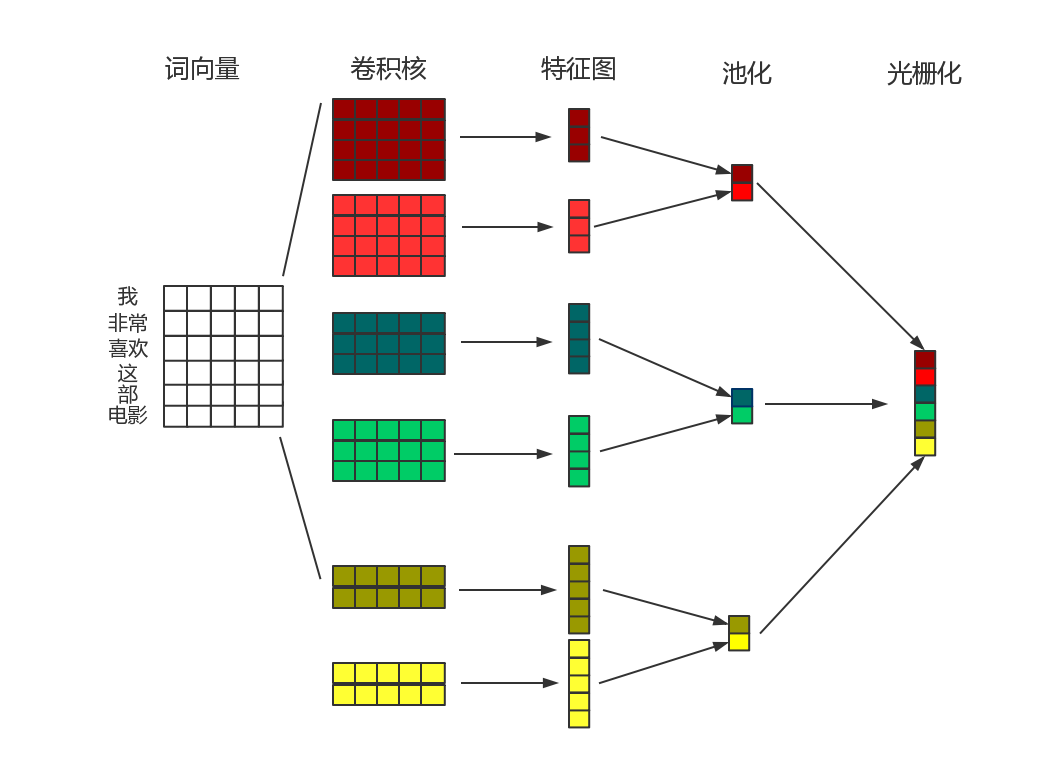
\includegraphics[scale=0.4]{picture/Text_CNN.png}
    \caption{卷积神经网络结构}
    \label{Text_CNN}
\end{figure}

(1)卷积层

卷积层主要用于特征提取,通过多个卷积核,对输入数据进行卷积计算,最后得到相应的特征图(Feature Map)。

卷积计算是通信领域中常见的计算方法,假设有二维离散函数$f\left ( x,y \right )$和$g\left ( x,y \right )$,
那么它们的卷积定义如公式\ref{cov_eqn}所示。
\begin{equation}
    f\left ( x,y \right )\ast g\left ( x,y \right )=\sum_{u}^{\infty }\sum_{v}^{\infty }f\left ( u,v \right )
g\left ( x-u,y-v \right )
    \label{cov_eqn}
\end{equation}

卷积核是提取特征的主要工具,相当于图像处理领域中的滤波器,
可以从输入数据中提取一类特征,其他类特征则需要另外的卷积核来提取,所以
卷积层通常包含有多个卷积核。一个卷积核包含参数矩阵$W$和偏置项$b$,计算过程如公式\ref{cov_layer_eqn}所示。
\begin{equation}
    h=f\left ( W\ast x+b \right )
    \label{cov_layer_eqn}
\end{equation}
其中$h$表示产生的特征图,$f$是激活函数。

具体到文本分类任务,输入数据为文本的词向量,
卷积核通常覆盖上下几行单词,并且宽度与词向量宽度相同(如图中卷积核部分所示),
这样就能够捕捉到多个连续词之间的语义特征,并且能够在同一类特征计算时共享参数。

(2)池化层(Pooling layer)

卷积层输出的特征图在数据纬度上与原始输入数据相比并没有减少很多,并且由于
存在多个卷积核,实际上输出数据往往会增多,如果不做处理,无疑会增加网络的复杂度,
产生巨大的计算量。

池化层也称为下采样层,在卷积层之后,对特征图进行降维操作(即池化操作)。
常见的池化操作有最大池化、最小池化和平均池化。其中最大池化是现在最常见的池化方式,
该方法将特征图分为多个子块,每个子块内部取最大的一个数据输出,
从而达到降低特征图纬度的目的。

对于文本数据,池化操作可以将长度不同的句子转化为长度相同的特征向量,方便后续统一处理。
另外最大池化还能够保留显著的特征。卷积核提取特征时,每一种卷积核会专注检测某一种含义的
词组,如果这种类型的词组出现了,该卷积核此时的输出值就会非常大,
通过最大池化就能够尽可能的将这些信息保留,同时忽略其他无关的信息。

(3)光栅层

输入数据经过卷积层与池化层计算之后,得到的是一系列特征图,而卷积神经网络之后的结构接收的
输入可能是一个特征向量。因此需要将这些特征图中的数据依次取出,排列成一个向量,
如网络结构图\ref{Text_CNN}中的光栅化部分所示。


\subsection{循环神经网络}
\label{rnn_section}
循环神经网络(Recurrent Neural Network,RNN)也叫做递归神经网络,是深度学习中另一个重要的网络模型。
RNN的结构如图\ref{RNN}所示,其特点是隐藏层节点不仅接收输入层的数据,还会接收上一个节点的输出数据作为另一个输入源,
这让RNN可以非常自然的处理序列数据,如文本、语音、视频等。
\begin{figure}[h]
    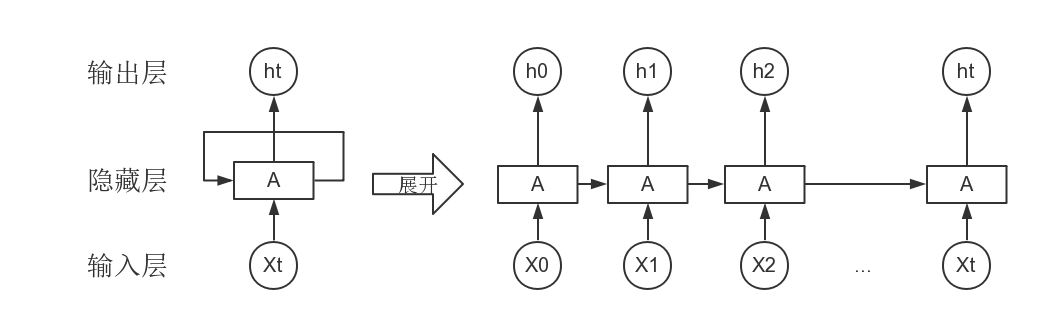
\includegraphics[scale=0.4]{picture/RNN.png}
    \caption{循环神经网络结构}
    \label{RNN}
\end{figure}
RNN中隐藏层节点包含三个部分,输入参数矩阵$U$、记忆参数矩阵$W$以及输出矩阵$V$,
对于节点$t$,计算公式如\ref{rnn_hidden_eqn}所示。
\begin{equation}
    s_t=f\left ( Ws_{t-1}+Ux_t \right )
    \label{rnn_hidden_eqn}
\end{equation}
其中$s_t$为中间向量,同时送往下一个隐藏层节点$t+1$与输出节点$h_t$,$f$一般为非线性激活函数
,$s_{t-1}$是上一个节点输出的中间向量。

对于文本分类任务,由于隐藏层中最后一个隐藏节点能够接收到之前所有节点的输出信息,
所以通常将该节点的输出向量作为网络最后生成的文本特征向量。

RNN模型的优点是对文本这类顺序数据有优秀的建模能力,能够突破n-gram模型中窗口大小的限制,
提取长间隔的单词之间的特征,
隐藏层最后一个节点的输出甚至可以包含前面所以单词的特征信息。
同时模型长度可变,对任意长度的文本都可以直接处理。

RNN模型的缺点也十分明显,那就是模型训练十分困难。根据反向传播算法,
RNN模型训练时会将梯度在隐藏层之间以乘积的形式传播,如果梯度大于$1$,
则多次相乘会使其指数级上升,引起梯度爆炸(Gradient Exploding);相反如果小于$1$,都次相乘后梯度逐渐为$0$,
又引起梯度消失(Gradient Vanishing)。

长短期记忆网络(Long Short Term Memory networks,LSTM)
\citing{hochreiter1997long}是对传统RNN模型的改进,
它将每个隐藏层节点看做“记忆细胞”,
在里面增加一种称为“门”的结构,对输入输出数据加以控制,从而有效解决梯度爆炸与梯度消失的问题。

LSTM的结构如图\ref{LSTM}所示,每个节点包含三个门结构(图中$\sigma $部分),
分别为遗忘门(Forget Gate)、输入门(Input Gate)与输出门(Output Gate)。
每个门由一个$Sigmoid$神经网络层和一个相乘操作组成,其中$Sigmoid$层输出$0\sim1$之间的值,
表示对应的部分信息是否应该通过,并利用相乘操作作用在输入或输出信息上,$0$值表示不允许信息通过,
$1$值表示让所有信息通过。
\begin{figure}[h]
    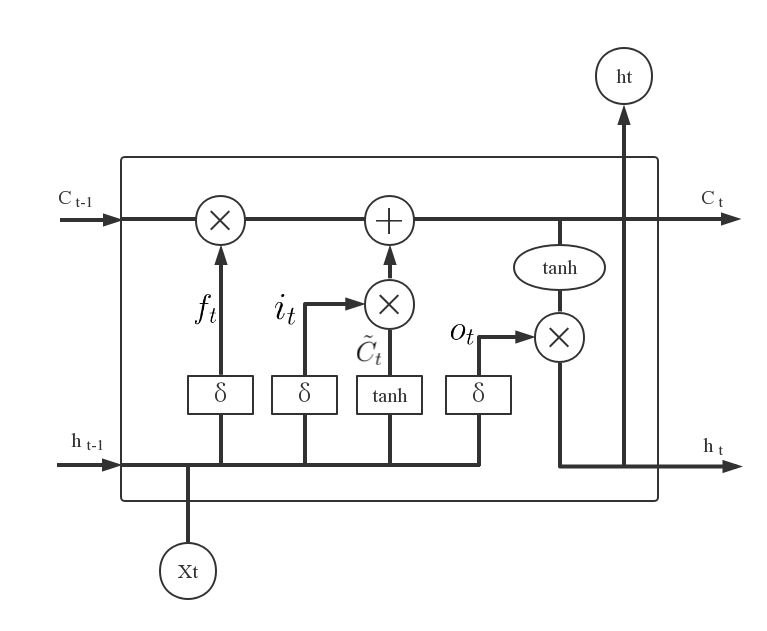
\includegraphics[scale=0.5]{picture/LSTM.png}
    \caption{长短期记忆网络}
    \label{LSTM}
\end{figure}

在一次计算过程中,LSTM节点首先计算遗忘门,公式如\ref{forget_gate_eqn}所示。
\begin{equation}
    f_t=\sigma\left ( W_f \cdot [h_{t-1},x_t]+b_f \right )
    \label{forget_gate_eqn}
\end{equation}

其中$W_f$与$x_t$是遗忘门中$Sigmoid$层的参数矩阵和偏置矩阵,$f_t$为遗忘向量,
里面的每一位都对应$C_{t-1}$中的一个数据,用来控制信息的流入。

第二步是将输入数据$x_t$存储到节点中,并更新节点状态。
这一步首先计算第二个门结构——输入门的$Sigmoid$层与一个tanh层,
得到两个候选值$i_t$与$\tilde{C}_t$,如公式\ref{input_gate_eqn}与\ref{input_gate_eqn2}所示。
\begin{equation}
    i_t=\sigma\left ( W_i \cdot [h_{t-1},x_t]+b_i \right )
    \label{input_gate_eqn}
\end{equation}
\begin{equation}
    \tilde{C}_t=\tanh\left ( W_C \cdot [h_{t-1},x_t]+b_C \right )
    \label{input_gate_eqn2}
\end{equation}

然后根据公式\ref{input_gate_eqn3}得到节点的新状态$C_t$。
\begin{equation}
    C_t=f_t \ast C_{t-1} + i_t \ast \tilde{C}_t 
    \label{input_gate_eqn3}
\end{equation}

最后,节点通过第三个门结构——输出门,得到输出向量,如公式\ref{output_gate_eqn}所示。
\begin{equation}
    \begin{split}
        o_t&=\sigma\left ( W_o \cdot [h_{t-1},x_t]+b_o \right ) \\
        h_t &= o_t \ast \tanh\left ( C_t \right )
    \end{split}
    \label{output_gate_eqn}
\end{equation}

通过增加门结构,LSTM有效避免了传统RNN在训练上的问题,但与CNN相比,
其训练效率依然十分低下,实际使用中常常造成问题。
因此,本文对短文分类算法的优化,将融合RNN与CNN,结合它们的优点,构建一个
对于中文短文快速有效的分类模型。

\section{本章小结}
本章首先对分词算法以及传统的文本表示方法与文本分类算法的基本理论做了简要介绍,
并指出了传统方法在中文短文本分类上的缺陷与不足。
接着引出了基于神经网络的短文本分类方法,详细介绍文本的词向量表示法以及
卷积神经网络和循环神经网络在文本分类任务中的应用。
这些基础内容为本文的后续工作提供了坚实的理论基础,后续章节将根据这些知识
搭建一个中文短文本分类模型。